% ############### 2.3) DEPLOYMENT VIEW ####################

In this section we describe the environment in which the system is executed from the perspective of the deployment diagram. Figure \ref{fig:deployment_diagram} shows the structure of the hardware components that execute the software, and presents the architecture in a more detailed way.


\begin{figure}[H]
    \makebox[\textwidth]{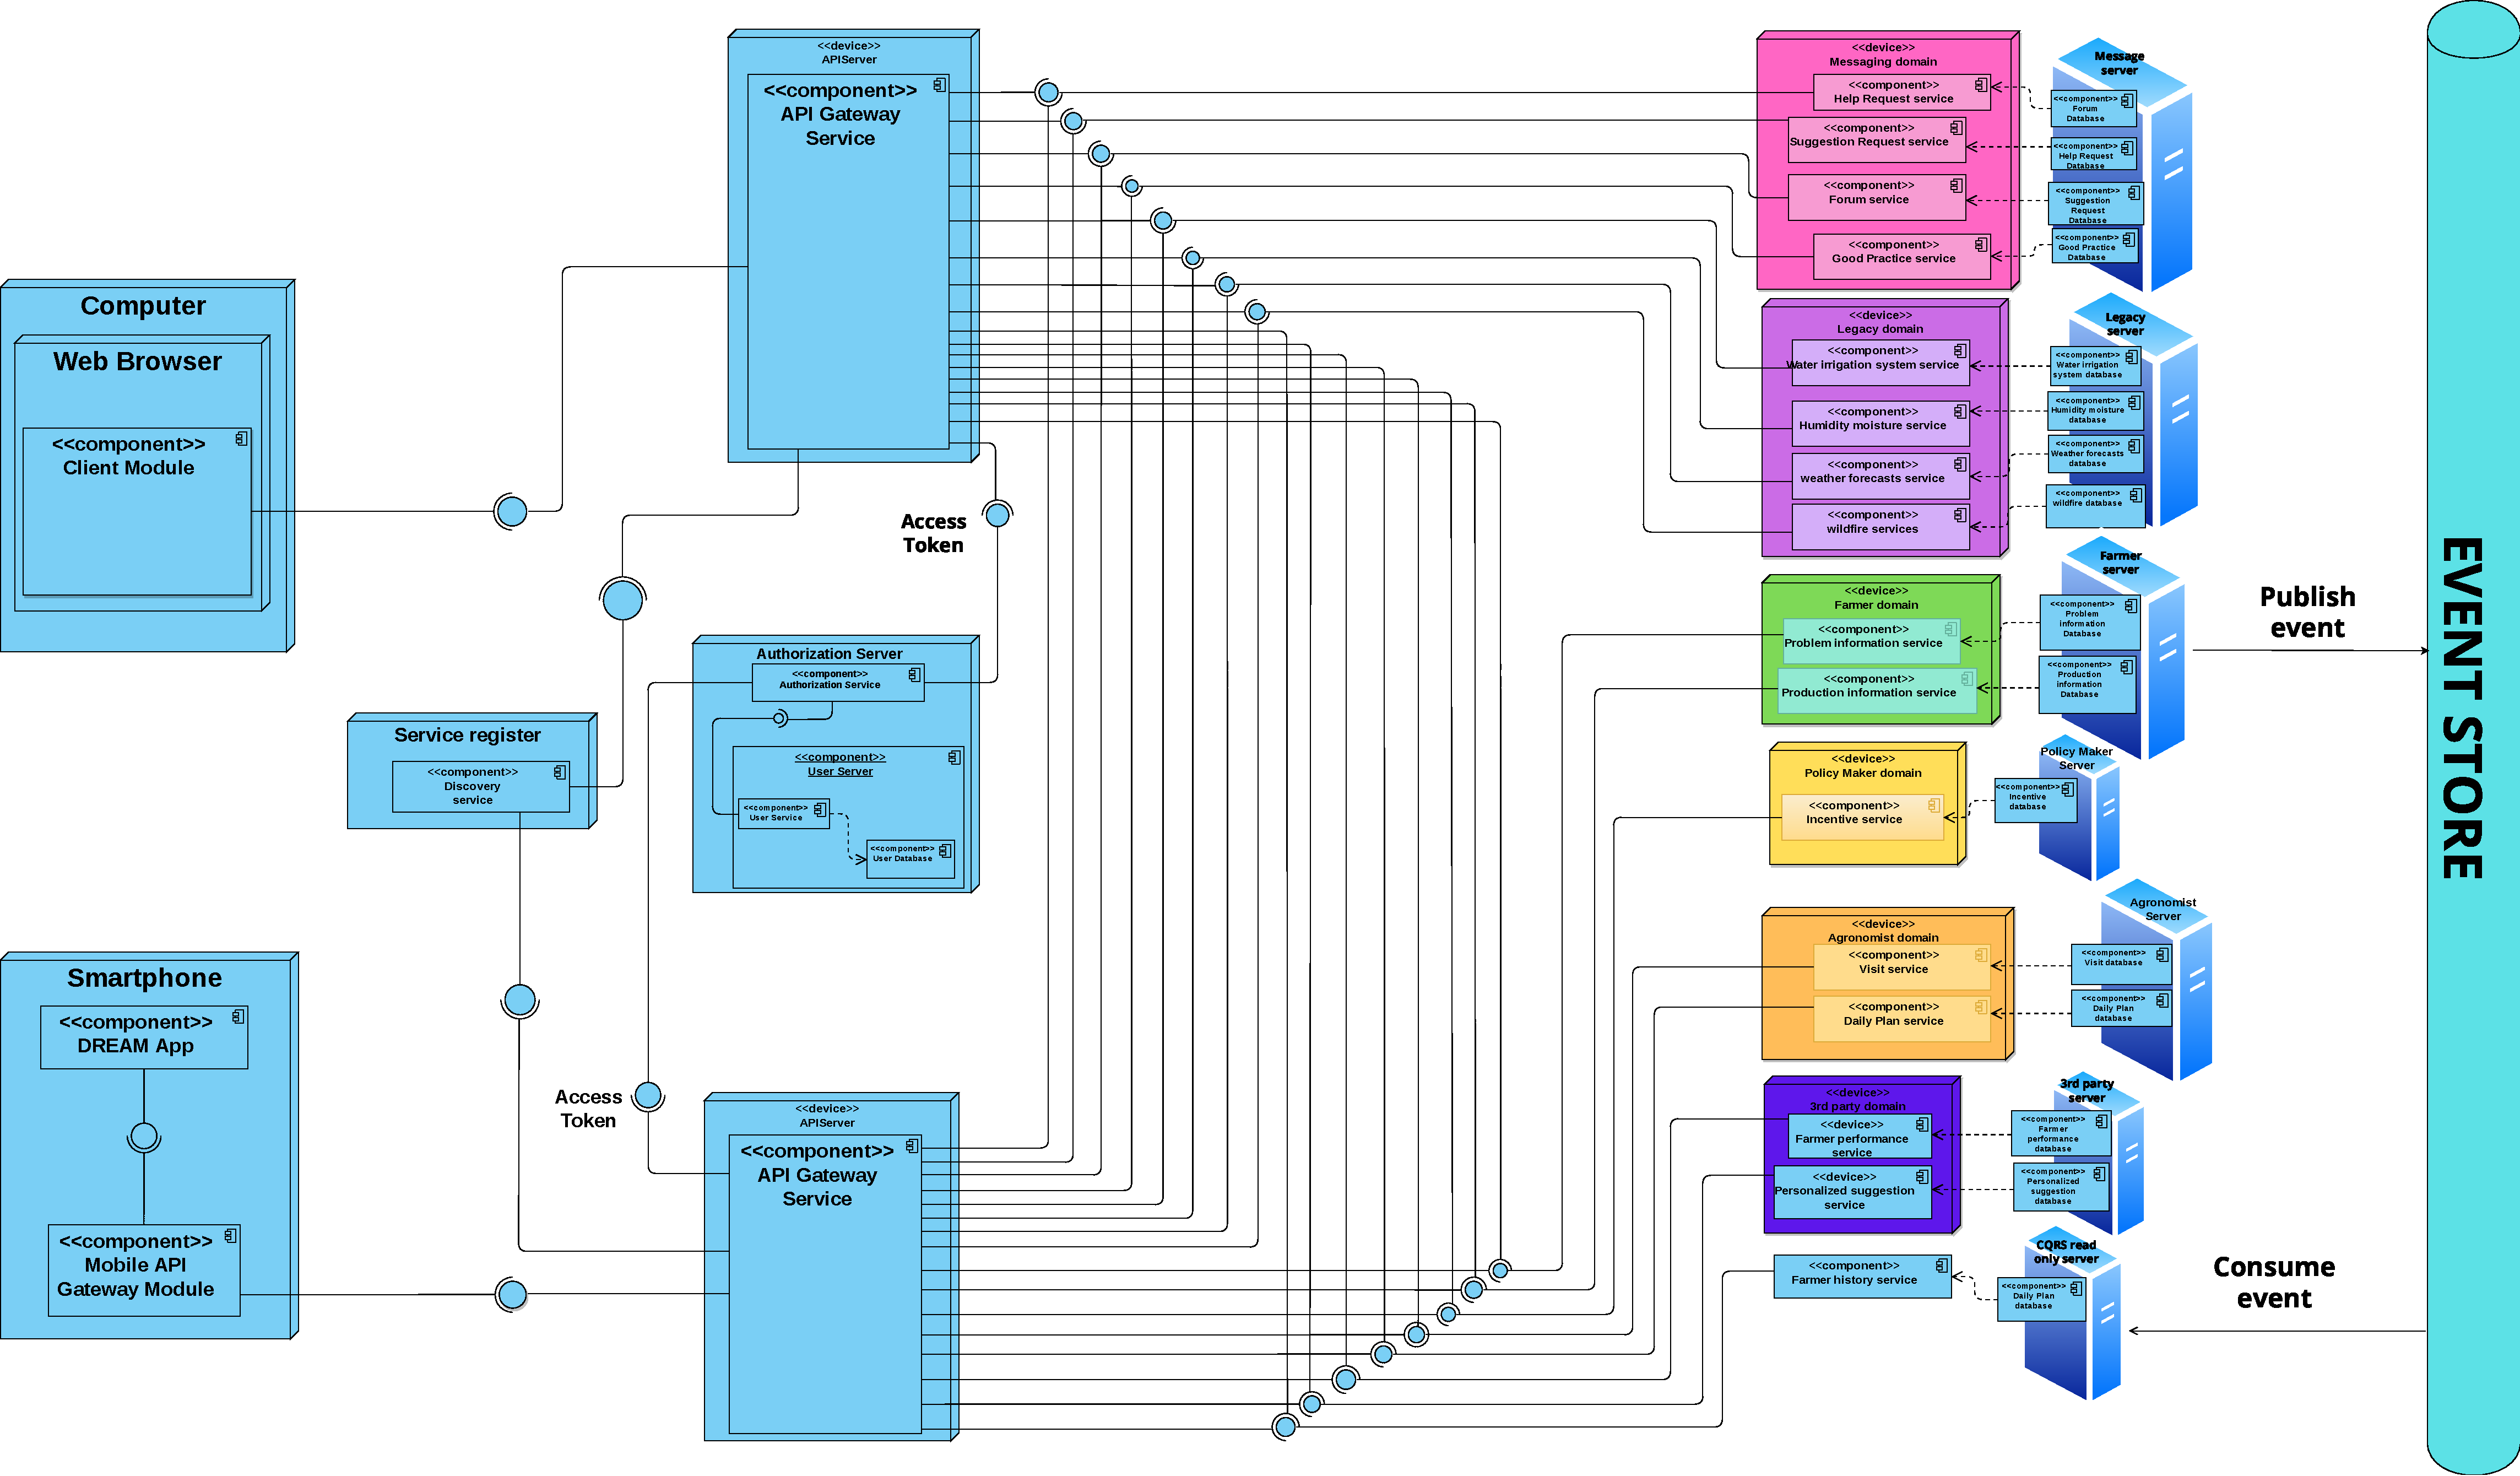
\includegraphics[width=\textheight, angle=90]{Images/deployment diagram.pdf}}
    \caption{\label{fig:deployment_diagram}Deployment diagram diagram}
\end{figure}

The above diagram highlights the four tiers of the architecture, and the relationship between components. In particular:
\begin{itemize}
    \item The \textsc{Presentation tier} is the front layer of the architecture and provides the final user interface (more details in section \ref{sect:user_interface_design}). As described in the RASD, the platform will be achievable through either an online web application or an installable mobile application. The web page's UI is supposed to provide both mobile and desktop visualization modes. This layer communicates with the application tier through API calls on HTTPS.
    \item The \textsc{routing tier} is composed by the API gateway pattern, which acts as the entry point of the application from the outer world. It is responsible mainly for request routing and protocol translation. It is similar to the Facade pattern from object-oriented design Like a facade, an API gateway encapsulates the application’s internal architecture and provides an API to its clients \cite{richardson2018microservices}. In addition to these functionalities, it is common practice to introduce in the API gateway pattern edge functionalities such as: authentication (Verifying the identity of the client making the request) and authorization (Verifying that the client is authorized to perform that particular operation) services, made possible through the introduction in the architecture of the authorization server component. Finally, in order to provide the service discovery pattern, a service registry component is required.
    \item The \textsc{business tier} contains the cloud of microservices that runs the core functionalities of the S2B. These ones are the same described in section \ref{sec:component_view} and communicate with the routing layer through RESTful APIs. Each microservice is responsible of a portion of the business logic and refer to its own database. Furthermore, microservices contained in the same domain (defined in the decomposition presented in section \ref{sec:component_view}) can be stored in the same server.
    \item Finally the \textit{data tier} contains the DBMS servers that store the data and provide SQL queries from the related microservices that communicate through an \textit{event store} for the implementation of the database management patterns (more details in section \ref{sec:styles_patterns}). This final tier could be implemented according to the \textbf{single service per container} or the \textbf{serverless} patterns.
\end{itemize}
